%%%%%%%%%%%%%%%%%%%%%%%% ExtendedAbstract.tex %%%%%%%%%%%%%%%%%%%%%%%%
%                                                                    %
%  Template for the 10-page extended abstract to be submitted for    %
%  the MSc degree conferral at Instituto Superior Tecnico.           %
%                                                                    %
%  Author:                                                           %
%                                                                    %
%       Andre C. Marta                                               %
%       Area Cientifica de Mecanica Aplicada e Aeroespacial          %
%       Departamento de Engenharia Mecanica                          %
%       Instituto Superior Tecnico                                   %
%       Av. Rovisco Pais                                             %
%       1049-001 Lisboa                                              %
%       Portugal                                                     %
%       Tel: +351 21 841 9466                                        %
%                        3466 (extension)                            %
%       Email: andre.marta@ist.utl.pt                                %
%                                                                    %
%  Created:       Dec  2, 2011                                       %
%  Last Modified: Dec 27, 2011                                       %
%%%%%%%%%%%%%%%%%%%%%%%%%%%%%%%%%%%%%%%%%%%%%%%%%%%%%%%%%%%%%%%%%%%%%%
% This document uses the LaTeX class file "article.cls"              %
%%%%%%%%%%%%%%%%%%%%%%%%%%%%%%%%%%%%%%%%%%%%%%%%%%%%%%%%%%%%%%%%%%%%%%
\documentclass[10pt,a4paper,twocolumn]{article}

%%%%%%%%%%%%%%%%%%%%%%%%%%%%%%%%%%%%%%%%%%%%%%%%%%%%%%%%%%%%%%%%%%%%%%
% Document preamble
%%%%%%%%%%%%%%%%%%%%%%%%%%%%%%%%%%%%%%%%%%%%%%%%%%%%%%%%%%%%%%%%%%%%%%

%% Builds upon the graphics  package, providing a key-value interface
%% for optional arguments to the \includegraphics command that go far
%% beyone what the graphics package offers.
%% http://www.ctan.org/tex-archive/help/Catalogue/entries/graphicx.html
%% if you use PostScript figures in your article
%% use the graphics package for simple commands
\usepackage{graphics}
%% or use the graphicx package for more complicated commands
%% \usepackage{graphicx}
%% or use the epsfig package if you prefer to use the old commands
%% \usepackage{epsfig}
\usepackage{graphicx} % Enhanced LaTeX Graphics

% Multiple figures
\usepackage{subfigure} % subcaptions for subfigures
\usepackage{subfigmat} % matrices of similar subfigures
\usepackage{multirow}
\usepackage{float}
\usepackage{caption}
\usepackage{stfloats}
\usepackage[table,xcdraw]{xcolor}
\usepackage{textcomp}

%Non-template packages
\usepackage{tikz}
\def\checkmark{\tikz\fill[scale=0.4](0,.35) -- (.25,0) -- (1,.7) -- (.25,.15) -- cycle;}
\usepackage{listings,xcolor}
\usepackage{xcolor}
\usepackage{multicol}
%adding urls to bibliography
\bibliographystyle{unsrtnat}
\usepackage[numbers]{natbib}
\usepackage{url}

% Declaring new column types
% 'dcolumn' package defines D to be a column specifier with
% three arguments: D{<sep.tex>}{<sep.dvi>}{<decimal places>}
%                  D{<sep.tex>}{<sep.dvi>}{<left digit places>.<right digit places>}
\usepackage{dcolumn}           % decimal-aligned tabular math columns
% d takes a single argument specifying the number of decimal places, e.g., d{2}
% or the number of digits to the left and right of the seperator, e.g., d{3.2}
\newcolumntype{.}   {D{.}{.}{-1}} % column alignedd on the point separator '.'
\newcolumntype{d}[1]{D{.}{.}{#1}} % column centered on the point separator '.'
\newcolumntype{e}   {D{E}{E}{-1}} % column centered on the exponent 'E'
\newcolumntype{E}[1]{D{E}{E}{#1}} % column centered on the exponent 'E'

%% American Mathematical Society (AMS) plain Tex macros
%%
%% The amsmath package is the principal package in the AMS-LaTeX distribution
%% http://www.ctan.org/tex-archive/help/Catalogue/entries/amsmath.html
\usepackage{amsmath}
%%
%% The amsfonts package provides extended TeX fonts
%% http://www.ctan.org/tex-archive/help/Catalogue/entries/amsfonts.html
\usepackage{amsfonts}
%% The amssymb package provides various useful mathematical symbols
\usepackage{amssymb}
%%
%% The amsthm package provides extended theorem environments
%% http://www.ctan.org/tex-archive/help/Catalogue/entries/amsthm.html
\usepackage{amsthm}

%% Improves the interface for defining floating objects such as figures and tables.
%% The package also provides the H float modifier option of the obsolete here package.
%% http://www.ctan.org/tex-archive/help/Catalogue/entries/float.html
\usepackage{float}

%% Control sectional headers. 
%% http://www.ctan.org/tex-archive/help/Catalogue/entries/sectsty.html
\usepackage{sectsty}
%%
%% Redefine the font size of the 'section' and 'subsection' headings
\newcommand{\myFontSize}{\fontsize{10}{0}\selectfont}
\sectionfont{\myFontSize}       % 10pt, Bold face (default)
\subsectionfont{\rm\myFontSize} % 10pt, Plain face

%% Select alternative section titles.
%% http://www.ctan.org/tex-archive/help/Catalogue/entries/titlesec.html
\usepackage{titlesec}
%%
%% Left indent, before and after spacing
%% (The starred version kills the indentation of the paragraph following the title)
\titlespacing*{\section}{0pt}{10pt}{0pt}
\titlespacing*{\subsection}{0pt}{10pt}{0pt}

%% Section numbers with trailing dots. 
%% http://www.ctan.org/tex-archive/help/Catalogue/entries/secdot.html
\usepackage{secdot}
%%
%% Also put a dot after the subsection number
\sectiondot{subsection}
%% Set a space between dot and heading text
\sectionpunct{section}{. }    % By default, \sectiondot places a \quad
\sectionpunct{subsection}{. } % after the number

% These are exact settings for a A4 page with top margin of
% 25 mm, bottom margin of 30 mm, left and right margins of 25 mm,
% printable area 242 X 160 mm.

\setlength{\topmargin}{-10.4mm}
\setlength{\headheight}{0.0mm}
\setlength{\headsep}{10.0mm}
\setlength{\textwidth}{160mm}
\setlength{\textheight}{242mm}
\setlength{\oddsidemargin}{0mm}
\setlength{\evensidemargin}{0mm}
\setlength{\marginparwidth}{0mm}
\setlength{\marginparsep}{0mm}

% New command to refer to equations as Eq.(1),Eq.(2),...
\newcommand{\eqnref}[1]{Eq.(\ref{#1})}

%%%%%%%%%%%%%%%%%%%%%%%%%%%%%%%%%%%%%%%%%%%%%%%%%%%%%%%%%%%%%%%%%%%%%%%%%%%%%%%%%%%%%%%%
% Title, authors and addresses

\title{Scalable web-based platforms for management of museological assets}
\date{October 2019}
\author{Duarte Miguel Ferreira Dias \\ duarte.ferreira.dias@tecnico.ulisboa.pt \\ \\ Instituto Superior T\'{e}cnico, Lisboa, Portugal}

%%%%%%%%%%%%%%%%%%%%%%%%%%%%%%%%%%%%%%%%%%%%%%%%%%%%%%%%%%%%%%%%%%%%%%%%%%%%%%%%%%%%%%%%
\begin{document}

% Begin one column section for title and abstract
%
% http://www.faqs.org/faqs/de-tex-faq/part5/
\twocolumn[
\begin{@twocolumnfalse}
\maketitle

%%%%%%%%%%%%%%%%%%%%%%%%%%%%%%%%%%%%%%%%%%%%%%%%%%%%%%%%%%%%%%%%%%%%%%
% ABSTRACT & KEYWORDS
%%%%%%%%%%%%%%%%%%%%%%%%%%%%%%%%%%%%%%%%%%%%%%%%%%%%%%%%%%%%%%%%%%%%%%
%%%%%%%%%%%%%%%%%%%%%%%%%%%%%%%%%%%%%%%%%%%%%%%%%%%%%%%%%%%%%%%%%%%%%%
%     File: ExtendedAbstract_abstr.tex                               %
%     Tex Master: ExtendedAbstract.tex                               %
%                                                                    %
%     Author: Andre Calado Marta                                     %
%     Last modified : 2 Dez 2011                                     %
%%%%%%%%%%%%%%%%%%%%%%%%%%%%%%%%%%%%%%%%%%%%%%%%%%%%%%%%%%%%%%%%%%%%%%
% The abstract of should have less than 500 words.
% The keywords should be typed here (three to five keywords).
%%%%%%%%%%%%%%%%%%%%%%%%%%%%%%%%%%%%%%%%%%%%%%%%%%%%%%%%%%%%%%%%%%%%%%

%%
%% Abstract
%%
\begin{abstract}

Asset management in museums has seen continuous improvements. With the advancements made in technology collection museums have evolved from using paper based registries to using digital systems that facilitate a collection manager's life as well the efficiency of performing modification to the asset base and registering these modifications.

Despite the currently available systems for asset management within museums, there is not a well defined best solution since these assets contain very diverse properties and requirements when cataloguing and storing their information.

The motivation for this work comes from the desire and necessity of creating a single highly adaptable and scalable solution capable of giving response to most museums.

This work has two main objectives: provide a long-term term solution that can be adapted for all museums to use in order to deal with their requirements when managing their collection of assets, and a short-term solution of providing a system capable of serving as a tool to solve IST's immediate need to catalogue its collection of assets from its multiple collections.

The motivation for the long-term objective comes with the current state of asset management solution, with most platforms providing a closed solution which is not meant to be adapted.

For the short-term objective, we are faced with IST, a university with a vast collection of assets from multiple areas which are not currently catalogued.

This work also provides insights into some of the currently used procedures when it comes to asset management within museums and how they differ from each other.
\\
%%
%% Keywords (max 5)
%%
\noindent{{\bf Keywords:}} Museum; Database; Asset Management; Extensibility; Web; Vue.js; Node.js; MongoDB \\

\end{abstract}



% End one column section (begin default two columns)
\end{@twocolumnfalse}
]
%%%%%%%%%%%%%%%%%%%%%%%%%%%%%%%%%%%%%%%%%%%%%%%%%%%%%%%%%%%%%%%%%%%%%%
% INTRODUCTION
%%%%%%%%%%%%%%%%%%%%%%%%%%%%%%%%%%%%%%%%%%%%%%%%%%%%%%%%%%%%%%%%%%%%%%
%%%%%%%%%%%%%%%%%%%%%%%%%%%%%%%%%%%%%%%%%%%%%%%%%%%%%%%%%%%%%%%%%%%%%%
%     File: ExtendedAbstract_intro.tex                               %
%     Tex Master: ExtendedAbstract.tex                               %
%                                                                    %
%     Author: Andre Calado Marta                                     %
%     Last modified : 27 Dez 2011                                    %
%%%%%%%%%%%%%%%%%%%%%%%%%%%%%%%%%%%%%%%%%%%%%%%%%%%%%%%%%%%%%%%%%%%%%%
% State the objectives of the work and provide an adequate background,
% avoiding a detailed literature survey or a summary of the results.
%%%%%%%%%%%%%%%%%%%%%%%%%%%%%%%%%%%%%%%%%%%%%%%%%%%%%%%%%%%%%%%%%%%%%%

\section{Introduction}
\label{Introduction}

Asset management is a crucial part of any museum. For a museum manager it is imperative to have the capability of inserting, viewing, editing and removing any asset at any given moment.


In the past, the main way of managing these assets was through paper registries, but with the emergence and development of information technologies we are now able to perform these task more efficiently and without as big of a risk of losing the information.

Despite the technological progress, there still isn't an ideal way of dealing with museological assets mainly due to their complexity and diversity. There exists already some software for performing these tasks but they are generally closed in the sense that the client is unable to adapt the platform to fit its specific needs.


The motivation for the development of this work comes with the anaylsis of a particular asset management case, more concretely, the one at Instituto Superior Técnico (IST). IST is a portuguese engineering college with a wide range of museological assets to manage, despite the lack of an estabilished system required to perform these necessary tasks.


As previously mentioned, one of the biggest challenges comes with the diversity of assets. IST is a perfect example of this scenario, having assets that range from rock and minerals all the way to motors and electronic devices. Another challenge comes with the lack of procedures which are currently not defined for IST.


Also, having an immediate need for such a management system, IST is the ideal case study to focus this work upon.


There already exist other systems in the market, such as closed-code products developed and sold by private companies, as well as opensourced solutions developed by the community. But still, with all the available solutions, none of them gives the necessary response to an institution such as IST.


%%%%%%%%%%%%%%%%%%%%%%%%%%%%%%%%%%%%%%%%%%%%%%%%%%%%%%%%%%%%%%%%%%%%%%
% BACKGROUND
%%%%%%%%%%%%%%%%%%%%%%%%%%%%%%%%%%%%%%%%%%%%%%%%%%%%%%%%%%%%%%%%%%%%%%
%%%%%%%%%%%%%%%%%%%%%%%%%%%%%%%%%%%%%%%%%%%%%%%%%%%%%%%%%%%%%%%%%%%%%%
%     File: ExtendedAbstract_backg.tex                               %
%     Tex Master: ExtendedAbstract.tex                               %
%                                                                    %
%     Author: Andre Calado Marta                                     %
%     Last modified : 27 Dez 2011                                    %
%%%%%%%%%%%%%%%%%%%%%%%%%%%%%%%%%%%%%%%%%%%%%%%%%%%%%%%%%%%%%%%%%%%%%%
% A Theory section should extend, not repeat, the background to the
% article already dealt with in the Introduction and lay the
% foundation for further work.
%%%%%%%%%%%%%%%%%%%%%%%%%%%%%%%%%%%%%%%%%%%%%%%%%%%%%%%%%%%%%%%%%%%%%%

\section{Background}

One of the difficulties of cataloguing the assets of museums comes with the vast amount of specific locations an asset can be in. Museums such as the museum of Geology and Mineralogy have most of their assets within cabinets, drawers and sections. This requires the documentation of the asset to be very precise in stating its location.

Another difficulty is related to the amount o properties associated to assets of different categories. The properties used to catalog and identify a painting and a mineral will be very different.

The thesis \cite{Barros2007MaterialidadeIST} developed by Miriam resulted on a Microsoft Access document with information on some of the assets of the museum of Geology and Mineralogy at IST. The document includes 3 different tables: identification, characteristics and history. These are the fields used to describe assets of this museum:

\vspace{4mm}
\textbf{Identification}
\begin{multicols}{2}
\begin{itemize}
    \item Inventory number
    \item Inventory A
    \item Inventory B
    \item Inventory C
    \item Designation 1
    \item Designation 2
    \item Designation 3
    \item Brand
    \item Collection
    \item Location
\end{itemize}
\end{multicols}
\vspace{4mm}
\textbf{Characteristics}
\begin{multicols}{2}
\begin{itemize}
    \item Inventory number
    \item Height
    \item Depth
    \item Diameter
    \item Weight
    \item Wood material
    \item Glass material
    \item Metal material
    \item Plastic material
    \item Other material
    \item Price
    \item Price assigner
\end{itemize}
\end{multicols}


\textbf{History}
\begin{multicols}{2}
\begin{itemize}
    \item Inventory number
    \item Acquisition date
    \item Acquisition method
    \item Acquisition price
    \item Supplier
    \item Conservation
    \item Repair
    \item Bibliography
    \item Exhibitions
    \item Sites 1
    \item Sites 2
    \item Sites 3
    \item Sites 4
    \item Documentation
\end{itemize}
\end{multicols}

\vspace{20mm}
\textbf{Spectrum}
\vspace{2mm}

%https://collectionstrust.org.uk/spectrum/spectrum-5/
Spectrum\cite{CollectionsTrust2009TheProcedure} is a collection management standard developed in the UK that is also used in other places around the world with the latest version having been published in September of 2017. According to its creators, Spectrum gives "tried-and-tested advice on the things most museums do when managing their collections".


This standard is activity-oriented, it focuses on how to register and execute certain activities, such as moving an object or updating location records. These activities are called procedures and Spectrum has a total of 21 defined procedures.


Each procedure has the following elements:

\begin{itemize}
    \item A definition that sums up the procedure into a single sentence.
    \item An explanation on the scope, explaining when the procedure should be used.
    \item The spectrum standard, that consists on the goal that we plan on achieving.
    \item A suggested workflow, this can be a diagram or a text written explanation.
\end{itemize}

When it comes to concrete procedures, these are the ones that Spectrum \cite{CollectionsTrust2009TheProcedure} considers to be its primary procedures:

\begin{itemize}
    \item Object entry - Registering incoming assets taking in to account the entry method (acquisition, loan, ...).
    \item Acquisition and accessioning - Taking legal ownership of objects in order to add them into the museum's collection.
    \item Location and movement control - Keeping track of the locations of all assets and updating them each time the assets are moved.
    \item Inventory - Making sure you have the basic information in order to identify your objects.
    \item Cataloguing - Managing the assets' information.
    \item Object exit - Recording when, the assets you are responsible for, exit your collection.
    \item Loans in - Managing objects you borrow for a fixed period of time and for a specific purpose.
    \item Loans out - Managing the requests for you to lend assets as well as the lending process until assets are returned to you.
    \item Documentation planning - Ongoing improvement of your documentation systems.
\end{itemize}

Taking this into account, Spectrum is not an all one single document but the composition of multiple documents, being that each one of these is associated to a specific procedure.


Spectrum is not a software itself but a set of rules that you should follow in order to create a digital of paper system that complies this management standard. There is not a single way of implementing this standard as we can see in the documents associated to the procedures, but as long as the base rules are followed we can consider a system to be compliant with this standard.

%%%%%%%%%%%%%%%%%%%%%%%%%%%%%%%%%%%%%%%%%%%%%%%%%%%%%%%%%%%%%%%%%%%%%%
% IMPLEMENTATION
%%%%%%%%%%%%%%%%%%%%%%%%%%%%%%%%%%%%%%%%%%%%%%%%%%%%%%%%%%%%%%%%%%%%%%
%%%%%%%%%%%%%%%%%%%%%%%%%%%%%%%%%%%%%%%%%%%%%%%%%%%%%%%%%%%%%%%%%%%%%%
%     File: ExtendedAbstract_imple.tex                               %
%     Tex Master: ExtendedAbstract.tex                               %
%                                                                    %
%     Author: Andre Calado Marta                                     %
%     Last modified : 27 Dez 2011                                    %
%%%%%%%%%%%%%%%%%%%%%%%%%%%%%%%%%%%%%%%%%%%%%%%%%%%%%%%%%%%%%%%%%%%%%%
% A Calculation section represents a practical development
% from a theoretical basis.
%%%%%%%%%%%%%%%%%%%%%%%%%%%%%%%%%%%%%%%%%%%%%%%%%%%%%%%%%%%%%%%%%%%%%%

\section{System Description}

The short term objective of this work is to provide a solution for IST's immediate need of being able to know what assets it currently owns. In order to do so, we require some minimum information such as the asset's identification/title, location and the collection it belongs to.

In the medium to long term, the objective of this work is to provide an easily scalable asset management platform where developers are capable of, without much effort or prior knowledge, adding new information specific to new groups of assets as well as adding other new features to the system. Another long term objective is to then integrate the platform with other applications besides the FenixEdu system.

The proposed platform will follow a web architecture as shown in figure \ref{webArchitecture}.

\begin{figure}[h!]
    \centering
    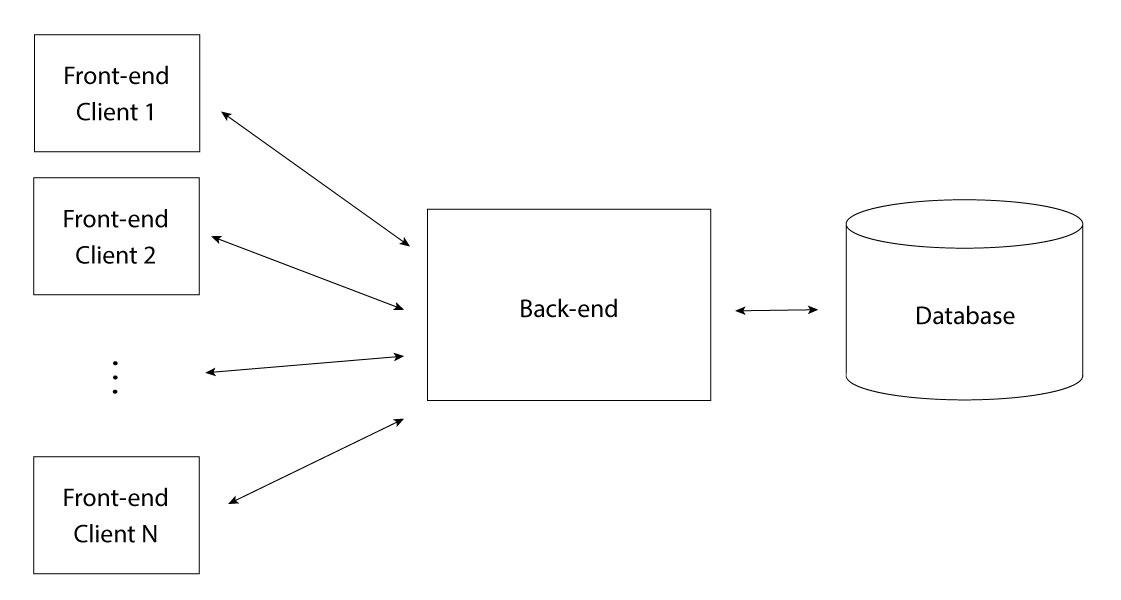
\includegraphics[scale=0.19]{images/Architecture/thesisArquitecture.jpg}
    \caption[Web architecture]{Commonly used web architecture that will serve as template for the platform.}
    \label{webArchitecture}
\end{figure}

%%%%%%%%%%%%%%%%%%%%%%%% DATA MODEL %%%%%%%%%%%%%%%%%%%%%%%%
\vspace{4mm}
\textbf{Data Model}
\vspace{2mm}

The main focus of this system is the way in which we will model our data. The most intuitive way of doing it would be having, for each asset, a node of information with all possible properties that the asset can have and only fill in the relevant properties for that specific asset. This would simplify our data structure since we would have the same structure for every single asset and would not have to create different structures for different assets. The problem here is that we would end up with vast amounts of irrelevant data fields as well as many properties without an associated value. 

A possible way of tackling this problem would be of creating a solution like the one presented in figure \ref{dataStructure1}.

\begin{figure}[h!]
    \centering
    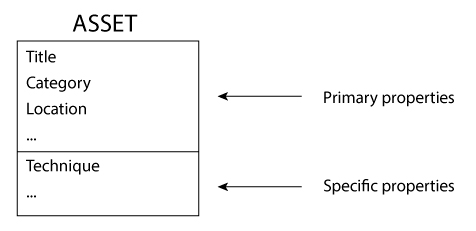
\includegraphics[scale=0.35]{images/Architecture/Data-structure-1.jpg}
    \caption[Data structure 1]{Initial data structure}
    \label{dataStructure1}
\end{figure}

In this data structure, we would define a couple of primary properties that would appear in all assets as well as a couple properties specific to the current asset. The specific properties would be conditional of the primary ones. This way, certain specific properties would be associated main properties' values. For example: an asset with the category of painting would only have, besides the primary properties associated to every assets, properties associated to paintings.

In this solution, an asset would have different sections (primary and specific ones) that are independent of each other. When relating this with the Spectrum standard \cite{CollectionsTrust2009TheProcedure} described in the previous chapter, we can divide each asset into multiple procedures where each procedure contains its properties. By doing this we are following the Spectrum standard as well and making the information associated to each procedure independent from each other.

\begin{figure}[h!]
    \centering
    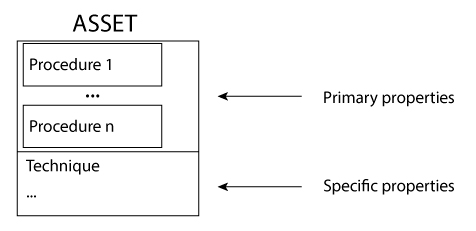
\includegraphics[scale=0.35]{images/Architecture/Data-structure-2.jpg}
    \caption[Data structure 2]{Spectrum procedure oriented data structure}
    \label{dataStructure2}
\end{figure}

Due to the limited timespan of this work, only a few key properties will be implemented. The chosen properties will be associated to the following groups and will provide IST with the minimum necessary information for cataloguing it's current asset collection:

\begin{itemize}
    \item Asset Identification
    \item Collection
    \item Asset Description
    \item Asset Location
    \item Asset History
\end{itemize}

Each one of these groups will include the minimum necessary information to identify an asset. These groups can be easily expanded to include more features as described in the full document of this work.

A possible solution for implementing the previously described data structure is JSON. JSON is a data format that allows for nesting variables, objects and arrays within each other, creating a simple to implement and read structure such as the tree associated to the specific properties. Another advantage of using JSON is the incorporation of this data format to other languages such as Javascript where a JSON element directly maps to a Javascript object \cite{Rischpater2015JavaScriptCookbook}.
    In listing \ref{assetJSON} an example of a possible asset JSON data structure is shown.
    
    \begin{lstlisting}[caption={Example of an asset's JSON data structure stored in the database.},label={assetJSON}]
{
    "_id" : 
    ObjectId("5d4d734bd1fa0"),
    "ObjectIdentification" : {
        "title" : 
        "Quadro da nascente",
        "optionalIds" : [
            {
                "N de inventorio B" : 
                "435"
            }
        ]
    },
    "ObjectDescription" : {
        "category" : [
            "Pinturas",
            "Gravuras"
        ]
    },
    "pinturas" : {
        "author" : "Eduardo Lopes",
        "year" : "2007",
        "material" : [
            "Madeira"
        ],
        "suporte" : "Madeira",
        "tecnica" : "Aguarela"
    },
    "gravuras" : {
        "amountOfCopies" : "252",
        "copyNumber" : "8"
    }
}
\end{lstlisting}

Specific modules can be associated to an asset depending on its category. In the previous listed example, we can observe that the data structure contains 2 objects which are conditionally inserted to the asset upon insertion: "pinturas" and "gravuras". The properties exist in the data structure since in the "ObjectDescription" both these properties are included. In this specific case "gravuras" is a sub-category of "pinturas", meaning that for an asset to have the property "gravuras" it must also have the property "pinturas".

%%%%%%%%%%%%%%%%%%%%%%%% DATA PERSISTENCE %%%%%%%%%%%%%%%%%%%%%%%%
\vspace{4mm}
\textbf{Data Persistence}
\vspace{2mm}

Now that the data structure is defined, we must ensure its persistance. This means that our data will survive even after the process that created it ends or if the system shuts down, to do so, a database is needed.

When thinking of a database choice in computer engineering the most popular option is using an SQL based system such as MySQL. A MySQL database is made up of multiple tables, with each table having a specific pre-defined data structure schema. In our museum example this means that we could have, for example, a table which contained all information of assets that were painting such as the author, technique, and so on. Each table then has rows, being that each row corresponds to a single item such as an asset. 

When looking into other database systems, another solution is using a document based database system such as MongoDB. In MongoDB, documents are grouped into collections, meaning that the database might have a collection for the assets, one for the users, and so on. When relating to MySQL, we can look at collections as being SQL tables and documents as being table rows. Documents follow a dynamic JSON structure, in this structure we can nest properties inside other properties \cite{MongoDB2016MongoDBGuide}. When comparing to the previously described SQL structure, in MongoDB collections do not have an associated data schema, meaning that they may contain assets with different properties. This solves the previously presented problems of using an SQL based system for managing museum assets.

In addition to this, the data model introduced in the previous section can be easily implemented by subdividing the content of each asset's documents into multiple independent modules.

%%%%%%%%%%%%%%%%%%%%%%%% BACK-END %%%%%%%%%%%%%%%%%%%%%%%%
\vspace{4mm}
\textbf{Back-end}
\vspace{2mm}

Having defined the data structure as well as the database the next step is to define how the necessary computing power will be implemented in order to perform operations on the database. Having users directly interacting with the database may bring problems such as data duplication or insertion of invalid data structures, which will compromise the whole system.

In order to prevent such problems a back-end infrastructure is defined. In this case, the back-end infrastructure will consist of the previously mentioned MongoDB database as well as a machine running processes capable of performing the standard database operations as well as ensuring the system's integrity.

An example such solution is using Node.js: an open-source, cross-platform JavaScript run-time environment that executes Javascript code outside of a browser in order to enable server-side scripting \cite{Corporation2019Node.jsGuide}. Since JSON and MongoDB documents perfectly map into Javascript objects, performing the necessary data conversions will be a seamless process. Throughout the rest of the work, this Node.js environment will be refered to as the back-end.

The back-end is based on routes which are identified by a unique URL according to the REST methodology \cite{GregorioIntroREST}. This means that in order for a user to interact with the system a request is sent, according to the REST API to the corresponding back-end route. So for example, in order to get the list of users in the database we will perform an HTTP GET request to a route similar to this one:

\textbf{GET}
\textbf{http://www.myServer.com/api/users}

Our back-end server will receive this request, access the database, insert all of the users into a javascript array and send that array to the front-end.

\begin{figure}[h!]
    \centering
    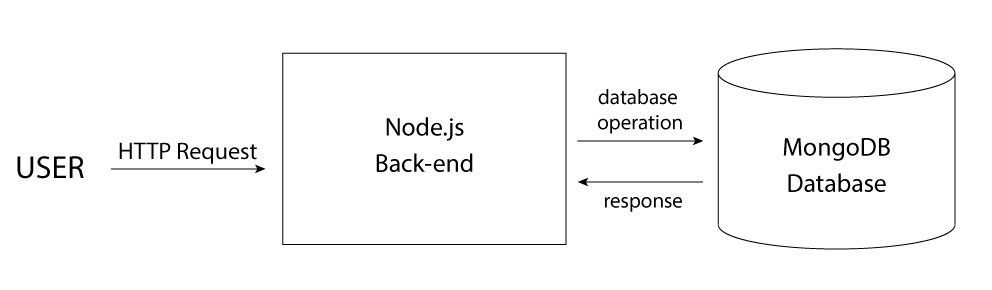
\includegraphics[scale=0.23]{images/Backend/backendRequest.jpg}
    \caption[Back-end request]{User performing a request to the back-end.}
    \label{backendRequest}
\end{figure}

This is a very basic example which does not include authentication. Security and user authentication will be discussed further on.

%%%%%%%%%%%%%%%%%%%%%%%% FRONT-END %%%%%%%%%%%%%%%%%%%%%%%%
\vspace{4mm}
\textbf{Front-end}
\vspace{2mm}

Performing an HTTP request to a web server requires some computer networking knowledge, leaving the system as it is now would only allow a reduced number of people to use it. It is possible to abstract all of the networking logic into something such as a browser interface with interactive buttons and data visualizations. This is called the front-end.

The front-end corresponds to the user interface with which the user will interact without the need of knowing any prior knowledge about programming. This is a case of code on demand, in order for the user to be able to use the platform we will simply need to open a web browser and type in the URL corresponding to the server directory in which the front-end files are stored. By doing this, the browser will send the necessary HTTP request to the server in order to get the interface code and will display it on the browser for the user to interact with.

In order to implement the front-end a framework called Vue.js (or simply Vue) can be used. Vue is a web development framework created by Evan You in 2013 after having worked for Google using the framework Angular.js in various projects. This framework allows us to separate the various parts of the platform into components. A component is a file which can contain HTML, CSS and Javascript code. We use components in order to better structure our code, it would be a mess if we had all the elements of our platform into the same HTML, CSS and Javascript files. Having the possibility of dividing the platform into components will prove to be very important in order to create a scalable code base where each element works independently from each other \cite{Copes2018VueHandbook}.

The code structure used for our front-end client is quite similar to the one seen in most Vue projects, the big difference is the way in which we use modules to create a truly dynamic and scalable platform. We define views that serve as the containers for other components but you can also look at views as if they correspond to each of our platform's different pages.

The big challenge with storing museological assets lies in their massive diversity of properties. It makes sense to specify what type of motor a car has but it does not make sense to specify what type of a motor a painting has. This is where our modules come in.

The main operations of the platform are the following:

\begin{itemize}
    \item Insert - Add a new asset to the database.
    \item Display - Observe an asset's details.
    \item Edit - Change an asset's details.
    \item Search - Search for assets with certain caracteristics.
    \item Config - Configure the values that a user can select for a specific module.
\end{itemize}

By defining these key operations we can now separate our assets' components into different modules. We have, for example, the object identification module which includes an asset's title and optional ids. For this module we will have insert, display, edit, search and config files.

\begin{figure*}[h!]
    \centering
    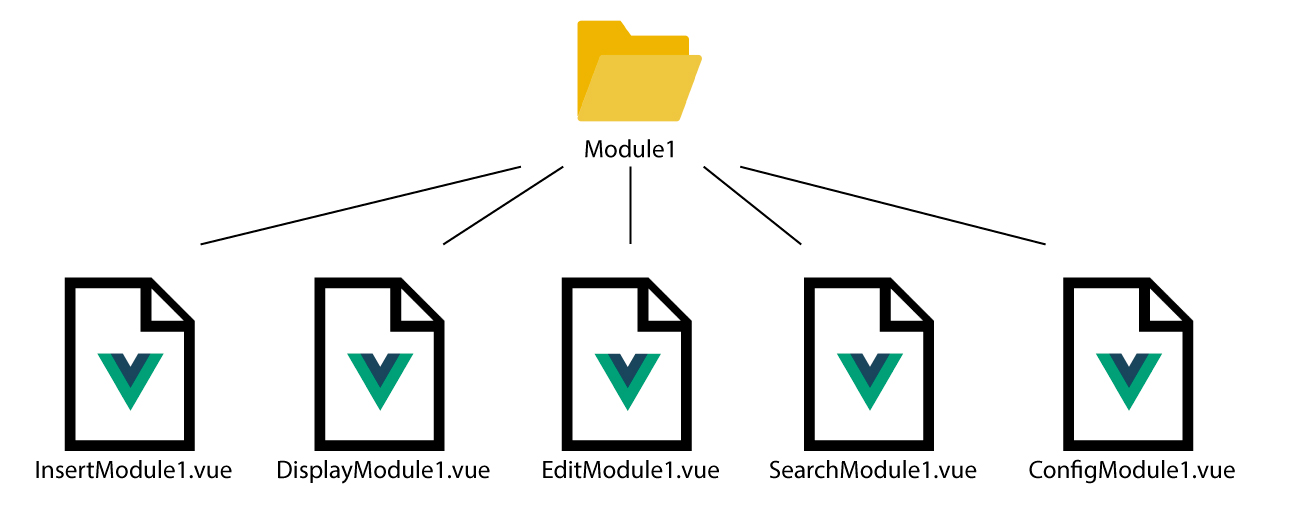
\includegraphics[scale=0.3]{images/Frontend/moduleStructure.jpg}
    \caption[Front-end module structure]{Module structure in front-end.}
    \label{moduleStructure}
\end{figure*}

This means that when displaying an asset we will render in our web page all of the modules relevant to the asset, thus creating a single information page that results from many Vue components. We can now also decide which modules we show to the user depending for each case. When displaying an asset we will view its categories and render all of modules corresponding to those categories if they exist, this is done dynamically in Vue by conditionally rendering Vue components.

In order to further illustrate the relation between a module and other components we can observe figure \ref{frontendStructure}.

\begin{figure}[h!]
    \centering
    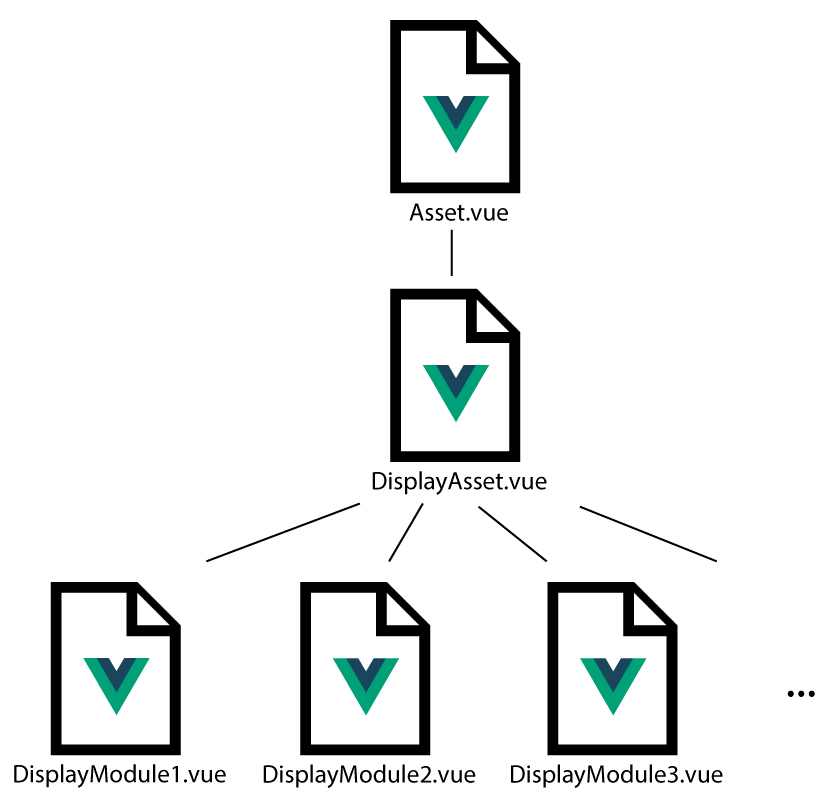
\includegraphics[scale=0.23]{images/Frontend/frontendStructure.jpg}
    \caption[Front-end file structure]{Example of how display modules are connected to parent components.}
    \label{frontendStructure}
\end{figure}

The front-end is tightly coupled to the back-end, meaning that it won't function properly without a running back-end server. Data that we view on the interface, such as the name of the assets, has to be fetched from the database. In order to get such data we perform HTTP requests to the back-end server. But using simple HTTP request is not enough since we want to load the data on the page dynamically and not have to refresh the page each time we make a request. For that we use AJAX in order to perform asynchronous requests to the server. An asynchronous operation allows us to perform other tasks while waiting for this operation to complete \cite{Gyorodi2016WebAjax}. After fetching the data, we can then process it and display it in our Vue component. Our system architecture will now resemble the one in figure \ref{exampleGET}.

\begin{figure}[h!]
    \centering
    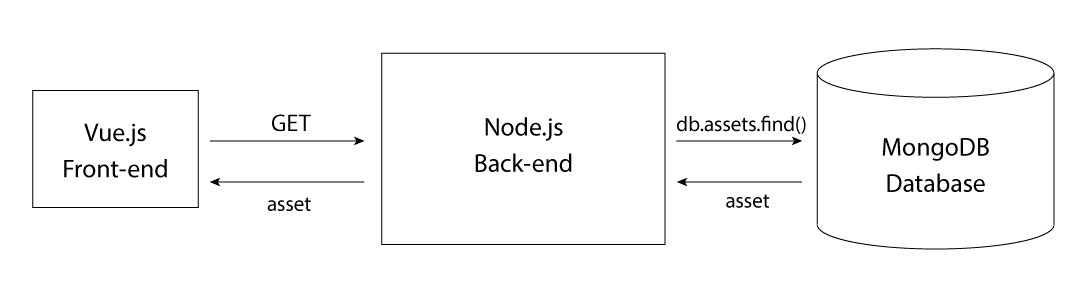
\includegraphics[scale=0.2]{images/Frontend/getAssetExample.jpg}
    \caption[Front-end request example]{Example of a client request for an asset.}
    \label{exampleGET}
\end{figure}

%%%%%%%%%%%%%%%%%%%%%%%% SECURITY AND AUTHENTICATION %%%%%%%%%%%%%%%%%%%%%%%%
\vspace{4mm}
\textbf{Security and Authentication}
\vspace{2mm}

Security is of key importance to our web platform since we have multiple users acessing common data on the database. We need to have a way of defining specific permissions for each user in order to control what they can and cannot do. We start by defining 3 types of possible user profiles:

\begin{itemize}
    \item Viewers - Can only view the assets in the database, they cannot change or delete anything.
    \item Editors - Can insert, edit and delete assets from the categories they have been assigned.
    \item Admins - Can do everything. This includes giving permissions to other users, configuring modules' data and inserting, editing and deleting any assets from the database.
\end{itemize}

To implement this security system we use JWT as well as the FenixEdu authentication system \cite{Silva2002TheProject} since we only want to allow users from IST to use our application for now.


JWT is used for passing tokens between machines in order to identify and validate who is sending the request \cite{Shingala2019JSONMQTT}. In our platform, the front-end will append a token to requests that require one. For example, editing is a higher permission feature which viewers must be unable to use. To make sure the person editing the asset can indeed do it we append a token that confirms the person's identity. Most requests such as a search query do not require the front-end to append a token to the message since every type of user can perform this action. Once the back-end receives a request, it will decode the token in order to identify the person performing the action. For this, it will need to know the secret with which the token was encrypted with, but that is no problem since the only entity that generates tokens is the back-end itself.

This is the authentication process:

\begin{enumerate}
    \item The front-end redirects the user to the FenixEdu login page.
    \item If the login is successfull, FenixEdu will redirect the user back to the front-end and append a code to the URL.
    \item The front-end sends a POST request to FenixEdu with the received code.
    \item FenixEdu responds with a token corresponding to the user's session.
    \item The front-end sends that token to the back-end
    \item The back-end gets the user's basic information from FenixEdu.
    \item The back-end checks if the user is already in the database, if not, a new user is created. The user university id is used as the user identifier.
    \item The back-end generates a jwt token and sends it as a response to the front-end.
    \item The front-end stores the jwt token locally and appends it to future requests when needed.
    \item Each time the back-end receives a jwt token, it decodes it and views if the user has the required permissions before continuing.
\end{enumerate}

The front-end checks, each time before we change pages, if the token is already in the front-end, if it is, the user will continue to the desired page. If not, the authentication process that can be seen in figure \ref{securityFlow} will be triggered in order to authenticate the current user.


\begin{figure}[h!]
    \centering
    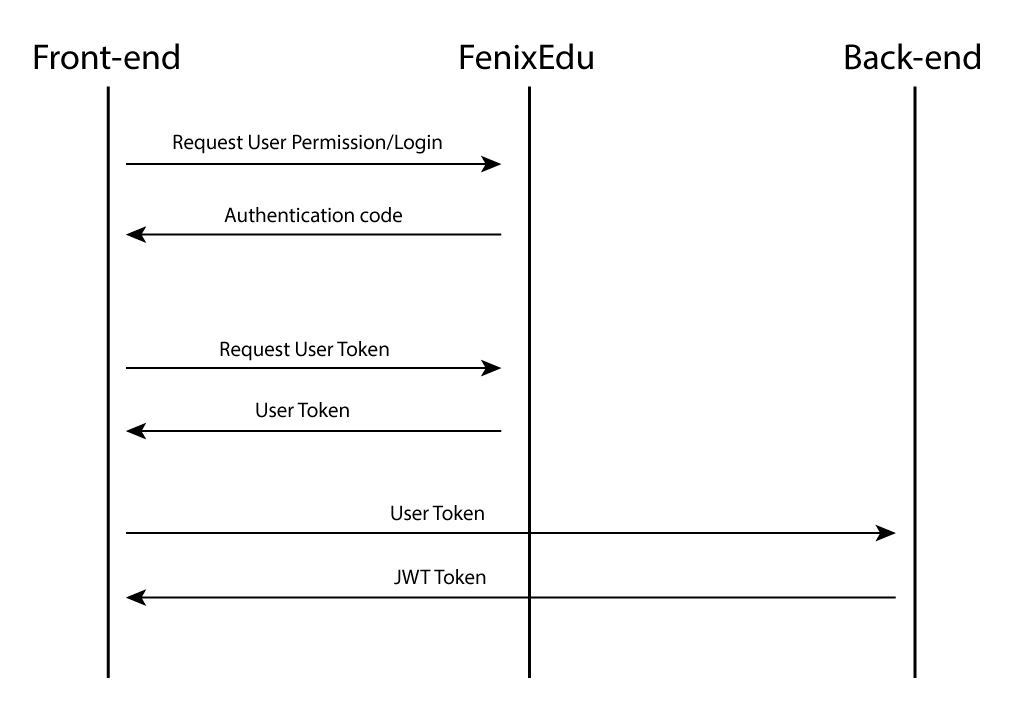
\includegraphics[scale=0.24]{images/Security/securityFlow.jpg}
    \caption[Login process]{User authentication process.}
    \label{securityFlow}
\end{figure}

%%%%%%%%%%%%%%%%%%%%%%%% CATEGORY MATCHING %%%%%%%%%%%%%%%%%%%%%%%%
\vspace{4mm}
\textbf{Category Matching}
\vspace{2mm}

In order to implement the dynamic modules previously described we require a way of identifying the categories of the asset. This information is included in the asset's JSON, more specifically in the Object Description object. In this object is included the information that associates the asset to certain categories in order to then allow for other dynamic modules to work. These categories follow a tree structure. This allows for the user to specify, within a category, the asset's sub categories in order to further identify the asset.
An example of a category tree is shown in figure \ref{paintingsTree}. In this example we can set an asset's category as being a painting and then drill down even further and state, for example, that it is also of the category acrylic.

\begin{figure}[h!]
    \centering
    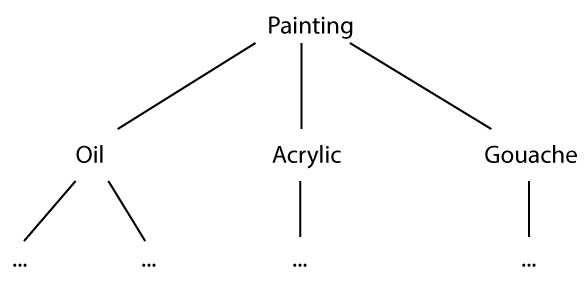
\includegraphics[scale=0.4]{images/Architecture/paintingsTree.jpg}
    \caption[Category tree example]{Example data structure of a category.}
    \label{paintingsTree}
\end{figure}

%%%%%%%%%%%%%%%%%%%%%%%% WEB PLATFORM %%%%%%%%%%%%%%%%%%%%%%%%
\vspace{4mm}
\textbf{Web Platform}
\vspace{2mm}

The work developed is based on a web architecture. This implies communication between machines, more concretely between: the front-end, back-end and database. Another option for this platform would be using other technologies to develop a solution with all of these 3 elements working locally in the same machine. Having a local solution would have its benefits when it comes to, for example, security since we would know exactly who could access the platform. The major drawback would be that the platform could only be accessed from a specific machine and only the people with access to that machine would be able to interact with our platform.


Right from the beginning it was known that this platform would have to be extremely convenient to use in order for museum collectors to make use of it. That is why the platform is based on a web architecture. This allows for collectors to manage their collections from any device and any place as long as they have an internet connection. Another advantage of having a web platform is that we can give the collectors the option of allowing the general public to view their collections without the ability to perform the same actions as the collection managers. But having these benefits comes with a price, and that is the need for more complex security systems in order to avoid that people who do not have permissions to edit the collections do so.


Another advantage of using a web platforms with these specific technologies is the ease of developing new features since javascript is currently one of the most popular programming languages amongst developers as well as being a higher-level programming language when comparing to others such as C or C++ in which the developers have to deal with concepts such as memory allocation and pointers which are abstracted in javascript.


When it comes to the choice of technologies for developing our web platform solution another choice of programming language would be using Python with, for example, the framework Django for the front-end and the framework Flask for the back-end \cite{Langtangen2015UsingApplications}. This would wield a very similar result, despite this observation, javascript was chosen for its popularity when it comes to web development since anyone with minimum knowledge of javascript would be able to quickly learn and implement small features in the current platform.

%%%%%%%%%%%%%%%%%%%%%%%%%%%%%%%%%%%%%%%%%%%%%%%%%%%%%%%%%%%%%%%%%%%%%%
% RESULTS
%%%%%%%%%%%%%%%%%%%%%%%%%%%%%%%%%%%%%%%%%%%%%%%%%%%%%%%%%%%%%%%%%%%%%%
%%%%%%%%%%%%%%%%%%%%%%%%%%%%%%%%%%%%%%%%%%%%%%%%%%%%%%%%%%%%%%%%%%%%%%
%     File: ExtendedAbstract_resul.tex                               %
%     Tex Master: ExtendedAbstract.tex                               %
%                                                                    %
%     Author: Andre Calado Marta                                     %
%     Last modified : 27 Dez 2011                                    %
%%%%%%%%%%%%%%%%%%%%%%%%%%%%%%%%%%%%%%%%%%%%%%%%%%%%%%%%%%%%%%%%%%%%%%
% Results
% Results should be clear and concise.
% Discussion
% This should explore the significance of the results of the work, not
% repeat them. A combined Results and Discussion section is often
% appropriate. Avoid extensive citations and discussion of published
% literature.
%%%%%%%%%%%%%%%%%%%%%%%%%%%%%%%%%%%%%%%%%%%%%%%%%%%%%%%%%%%%%%%%%%%%%%

\section{System Validation}

In order to achieve the short-term objective of this work of cataloguing the current assets at IST we will now look into how the current existing asset repositories can be included into the developed system.

These are the properties developed during the timeframe of this work:

\begin{itemize}
    \item Asset Identification
    \begin{itemize}
        \item Title
        \item Inventory numbers
    \end{itemize}
    \item Collection
    \begin{itemize}
        \item Collection name
    \end{itemize}
    \item Asset Description
    \begin{itemize}
        \item Category name
    \end{itemize}
    \item Asset Location
    \begin{itemize}
        \item IST location (current and usual)
        \item Coordinates (current and usual)
        \item Address (current and usual)
    \end{itemize}
    \item Asset History
    \begin{itemize}
        \item Event name
        \item Event description
        \item Event date
    \end{itemize}
\end{itemize}

\vspace{4mm}
\textbf{IST general inventory sheet}
\vspace{2mm}

When looking into assets that follow the structure of a common IST physical asset information sheet presented in this work's full document, it is possible to create a direct mapping between some of the properties. These are the properties lost when inserting the asset into the platform:

\begin{multicols}{2}
\begin{itemize}
    \item Description
    \item Brand
    \item Date
    \item Image id
    \item Dimensions
    \item Material
    \item Price evaluation
\end{itemize}
\end{multicols}

All of these properties can be stored within the platform by extending it with the implementations of new modules.

\vspace{4mm}
\textbf{Paintings sheets}
\vspace{2mm}

When looking into assets that follow the structure of a painting asset sheet at IST presented in this work's full document, it is also possible to establish a mapping between the properties of the inventory sheet and the platform. In this case all of the properties can be included into the platform since specific modules were developed for these categories of asset, more specifically the modules "Pintura" and "Gravura".

This is a good example of how, by extending the platform, as seen in the previous chapters, we are able to store all information relative to any type of asset category.

\vspace{4mm}
\textbf{Museum of geology and mineralogy}
\vspace{2mm}

As previously mentioned, the museum of geology and mineralogy has a Microsoft Access information with information of some of its assets. These assets have properties divided into 3 groups:

\begin{itemize}
    \item Identification
    \item Characteristics
    \item History
\end{itemize}

In the Identification group all properties are covered except the asset brand.
In the Characteristics and History groups most properties are not covered by the platform, in order to incorporate them the platform needs to be extended with new modules similarly to what was done with the paintings.


%%%%%%%%%%%%%%%%%%%%%%%%%%%%%%%%%%%%%%%%%%%%%%%%%%%%%%%%%%%%%%%%%%%%%%
% CONCLUSIONS
%%%%%%%%%%%%%%%%%%%%%%%%%%%%%%%%%%%%%%%%%%%%%%%%%%%%%%%%%%%%%%%%%%%%%%
%%%%%%%%%%%%%%%%%%%%%%%%%%%%%%%%%%%%%%%%%%%%%%%%%%%%%%%%%%%%%%%%%%%%%%
%     File: ExtendedAbstract_concl.tex                               %
%     Tex Master: ExtendedAbstract.tex                               %
%                                                                    %
%     Author: Andre Calado Marta                                     %
%     Last modified : 27 Dez 2011                                    %
%%%%%%%%%%%%%%%%%%%%%%%%%%%%%%%%%%%%%%%%%%%%%%%%%%%%%%%%%%%%%%%%%%%%%%
% The main conclusions of the study presented in short form.
%%%%%%%%%%%%%%%%%%%%%%%%%%%%%%%%%%%%%%%%%%%%%%%%%%%%%%%%%%%%%%%%%%%%%%

\section{Conclusions}

%%%%%%%%%%%%%%%%%%%%%%%% EXTENSIBILITY %%%%%%%%%%%%%%%%%%%%%%%%
\vspace{4mm}
\textbf{Extensibility}
\vspace{2mm}

In order to evaluate the extensibility of the platform, the code base was provided to a developer in order for him to develop a new module for the system. The developed module corresponds to the historical events associated to an asset where the user is capable of inserting the start and end time of the event, the event name and the event description. This means that if, for example, there happens to be an asset that was in exhibition at some specific place and time the platform user is capable of recording this information.

The developer assigned to developing this new module had never seen the platform before and was just given the technical guide in chapter 3 of this work's full document. The developer, who is called Artur, was at the time of this work a computer science student in his first year of his masters degree at IST with some experience in Vue, Node.js and Javascript.

In these conditions, Artur was capable of fully developing this new module in 1 hour and 38 minutes. The module includes insertion, display, editing and search.

Given the short amount of time required for a developer with absolutely no knowledge of the platform to develop a new module, we can conclude that the platform allows for fast and easy development of new components.

%%%%%%%%%%%%%%%%%%%%%%%% EXTENSIBILITY AUTOMATION %%%%%%%%%%%%%%%%%%%%%%%%
\vspace{4mm}
\textbf{Extensibility Automation}
\vspace{2mm}

Being this a platform that provides developers with a straightforward and repeatable guide on how to implement new modules, it should be possible to develop software to, given the new module's description, create new components automatically without requiring any coding. This was not implemented in this work due to the limited time frame but by implementing a script that will follow the technical guidelines given in chapter 3, the museums owner is able to adapt the platform to its specific needs without the need of any coding or knowledge on how the platform is implemented.

%%%%%%%%%%%%%%%%%%%%%%%% FINAL THOUGHTS %%%%%%%%%%%%%%%%%%%%%%%%
\vspace{4mm}
\textbf{Final Thoughts}
\vspace{2mm}

This thesis had two main objectives, one is for the short-term and the other for the long-term.

The short-term objective was to provide an immediate solution for managing the assets at IST. To achieve this, a web platform was developed with the features needed to properly identify different assets from different collections as well as other important information associated to them such as their current location. The platform provides essential operations including: insertion of an asset, visualization of an asset's information, capability of editing an asset's information upon insertion, ability to search within the platform in order to find specific assets and configuring what values can be selected from specific asset properties upon asset insertion, editing and searching.

The long-term objective was to provide the foundations for an extensible asset management system so that anyone with minimal programming knowledge can develop further components for it in order to fit any necessary requirements for other museums. To achieve this, a web platform capable of managing assets was developed, the same one described in the short-term objective. The architecture of this platform was developed in a way that allows for an ease of extensibility by modularizing its components so that new developments remain independent from previously defined ones. To add to this architecture, a step by step technical process on how to develop new modules for the platform was written in order to allow developers with little knowledge of Javascript to develop these new modules.

The initial study also raised attention to the importance of the use of proper asset management systems for museums in order to maintain their collections visible and accessible for people to see. In an institution such as IST where the assets are not catalogued neither publicly available, having a digital system to manage the assets might lead to a better internal knowledge of what assets exists as well as facilitate the public sharing of information regarding its collections and exhibitions.

%Future work
The developed platform is far from being a finished product, but it is the foundation where other developers can create more functionalities and features in order to possibly create multiple solutions for multiple different museums.

%%%%%%%%%%%%%%%%%%%%%%%%%%%%%%%%%%%%%%%%%%%%%%%%%%%%%%%%%%%%%%%%%%%%%%
% REFERENCES
%%%%%%%%%%%%%%%%%%%%%%%%%%%%%%%%%%%%%%%%%%%%%%%%%%%%%%%%%%%%%%%%%%%%%%

% Produces the bibliography section when processed by BibTeX
%
% Bibliography style
% > entries ordered alphabetically
%\bibliographystyle{plain}
% > unsorted with entries appearing in the order in which the citations appear.
%\bibliographystyle{unsrt}
% > entries ordered alphabetically, with first names and names of journals and months abbreviated
\bibliographystyle{ieeetr}
% > entries ordered alphabetically, with reference markers based on authors' initials and publication year
%\bibliographystyle{alpha}

% External bibliography database file in the BibTeX format (ExtendedAbstract_ref_db.bib)
\bibliography{mendeley_v2.bib}

%%%%%%%%%%%%%%%%%%%%%%%%%%%%%%%%%%%%%%%%%%%%%%%%%%%%%%%%%%%%%%%%%%%%%%
\end{document}
%%%%%%%%%%%%%%%%%%%%%%%%%%%%%%%%%%%%%%%%%%%%%%%%%%%%%%%%%%%%%%%%%%%%%%

